API stands for Application Programming Interface. An API is a set of routines, protocols, and tools for building software applications. The API specifies how software components should interact and are used when programming graphical User Interface (GUI) components. A good API makes it easier to develop a program by providing all the building blocks. A programmer then puts the blocks together.

In this project the API will be induced between the MCTS algorithm i.e. AI and the board game application. It will be responsible for providing the input to the board game application in understandable format and will receive the input from the MCTS algorithm. Its usage is described in figure \ref{fig:flowchart}.
\newpage


\begin{figure}[H]
	\centering
	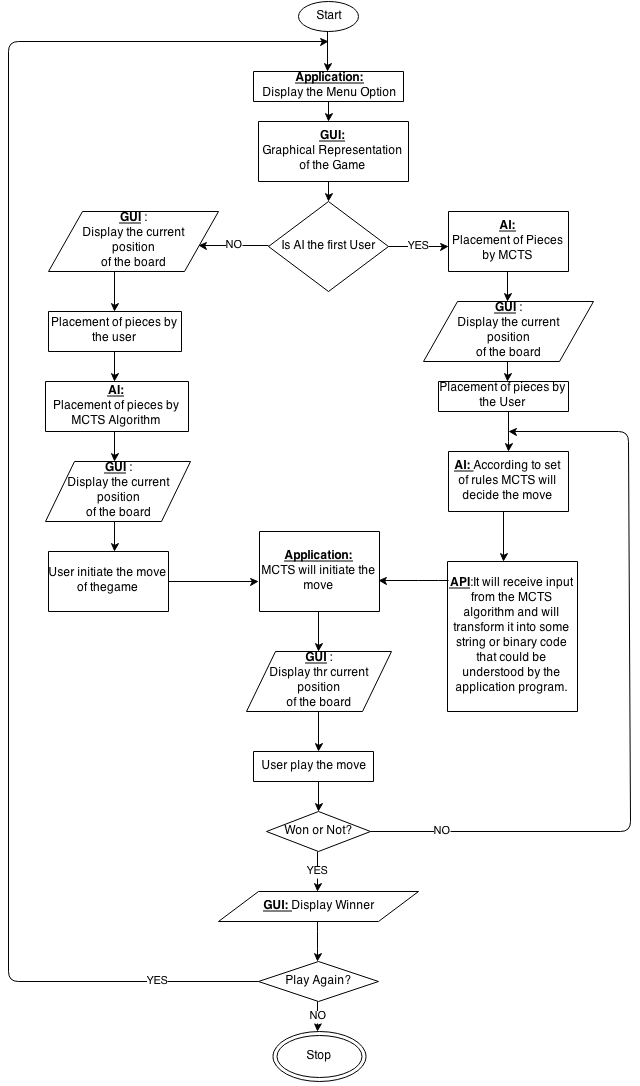
\includegraphics[width=0.8\textwidth]{2General_Architecture/2.2API/img/DiagramAPI.png}
	\caption{The flowchart describing the usage of the API}
	\label{fig:flowchart}
\end{figure}
\thispagestyle{empty}

